\definecolor{listingBackground}{rgb}{0.95,0.95,0.95}
\lstset{language=Prolog, 
		backgroundcolor=\color{listingBackground},
		numbers=left,
		numberstyle=\footnotesize,
		breaklines=true,
		breakautoindent=true,
		postbreak=\space,
		tabsize=2,
		basicstyle=\ttfamily\footnotesize,
		showspaces=false,
		showstringspaces=false,
		stepnumber=2,
		numbersep=5pt,
		keywordstyle=\color{red}\bfseries\emph,
		keywordstyle=[2]\color{cyan}\ttfamily,
		frame=single,
		inputencoding=latin1,
		extendedchars=true,
		captionpos=b, 
		morekeywords={connectedHV,distance,abs},
		morekeywords=[2]{S,S1,S2,P,P1,P2,X,X1,X2,Y,Y1,Y2},
		otherkeywords={:-,.},
		commentstyle=\color{MidnightBlue}\emph,
		stringstyle=\color{cyan}	
	}
\subsection{Client - Prolog} \label{sec:Prologclient}
	Die Aufgaben des Prolog-Clients sind in verschiedene Module unterteilt, um die verschiedenen Teile austauschbar zu halten. 
	Abbildung \ref{fig:prologmodule} zeigt das Zusammenspiel der Module. Dabei stellt ein Pfeil die Verwendung eines Prädikates aus
	dem jeweiligen Modul dar. Die im Diagramm dargestellten Pfeile zeigen somit die Schnittstellen zwischen den Modulen auf.
	
	\begin{figure}[H] % (fold)
		\centering
		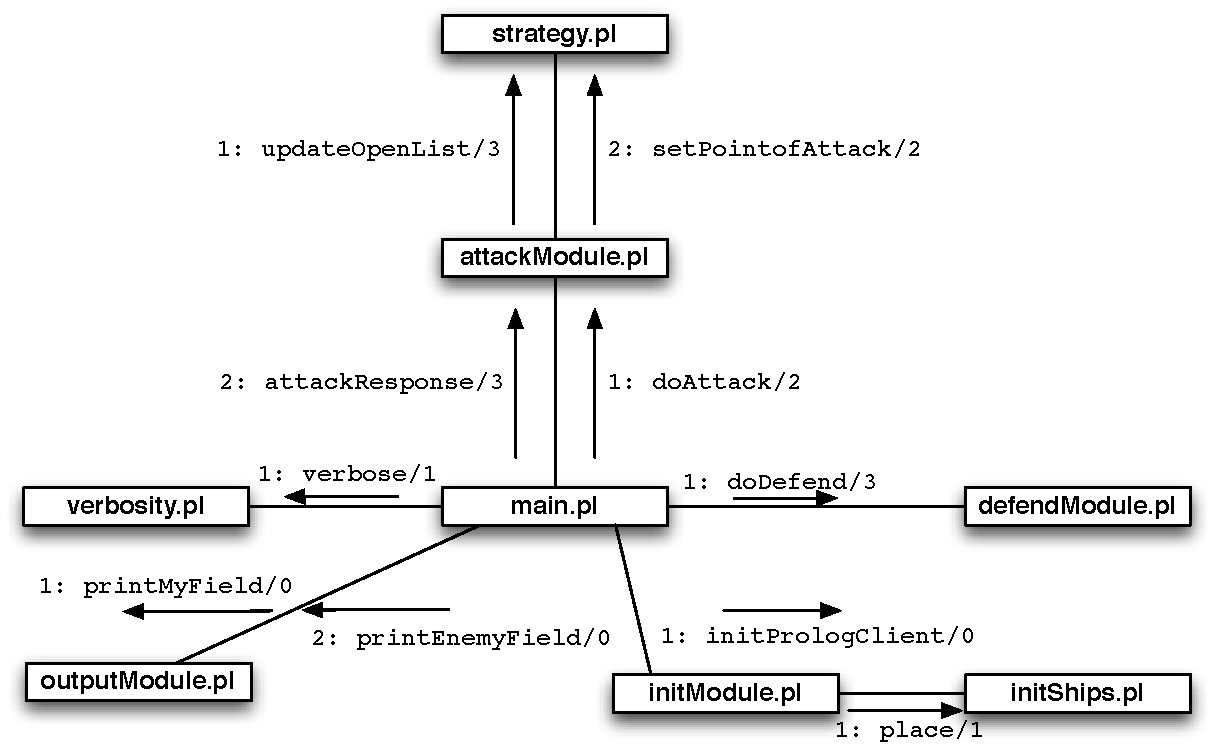
\includegraphics[width=0.9\textwidth]{images/ModuleCommunication.pdf}
		\caption{UML Kommunikationsdiagramm zur Kommunikation zwischen den Modulen des Prolog-Clients}
		\label{fig:prologmodule}
	\end{figure}
	% figure fig:prologmodule (end)

	Des Weiteren arbeiten einige der Module gemeinsam auf \textit{globalen} Spielvariablen, die mit Hilfe von dynamischen Prädikaten
	gespeichert werden. Tabelle \ref{tbl:globalevariablen} zeigt diese Variablen, ihren Zweck sowie ihre Verwendung auf.
	
	%\begin{table}[H]
	%	\centering
		\begin{longtable}{|l|p{6cm}|p{5cm}|}
			\hline
			Prädikat & Zweck & Verwendet von \\ 
			\hline 
			\hline \endhead
			\texttt{myField/1} & Speichert Zustand des eigenen Spielfeldes & Initialisierungsmodul, Verteidigungsmodul, Ausgabemodul \\
			\hline
			\texttt{enemyField/1} & Speichert Zustand des gegnerischen Spielfeldes & Initialisierungsmodul, Strategiemodul, Angriffsmodul, Ausgabemodul \\
			\hline
			\texttt{openList/1} & Speichert Liste der bevorzugt anzugreifenden, gegnerischen Felder & Initialisierungsmodul, Strategiemodul, Ausgabemodul \\
			\hline
			\texttt{numberOfGames/1} & Speichert Verbleibende Anzahl von Spieldurchgängen (für aufeinander folgende Durchgänge) & Hauptmodul \\
			\hline
			\texttt{numberOfWins/1} & Speichert die Anzahl der bisher gewonnenen Spiele (für aufeinander folgende Durchgänge) & Hauptmodul \\
			\hline
			\texttt{numberOfLosses/1} & Speichert die Anzahl der bisher verlorenen Spiele (für aufeinander folgende Durchgänge) & Hauptmodul \\
			\hline
			\texttt{currentStream/1} & Speichert den aktuell gesetzten Ausgabestrom (Konsole, Datei, keiner) & Hauptmodul, Ausgabemodul \\
			\hline
%		\end{tabular}
		\caption{Prädikate für globale Spielvariablen}
		\label{tbl:globalevariablen}
	\end{longtable}
	
	Im Folgenden werden die Aufgaben und die Funktionsweise der verschiedenen Module erläutert.

\subsubsection{Hauptmodul} \label{sec:hauptmodul}
	Das Hauptmodul \texttt{main.pl} wird beim Starten des Clients aufgerufen. Der Client bietet die Möglichkeit eine konfigurierbare Anzahl
	von Runden zu spielen. Dies wird vorallem bei Spielen verwendet, in denen zwei \textit{Computergegner} gegen einander antreten. 
	Beim Start des Clients werden deshalb zunächst die Anzahl der Spiele, Siege sowie Niederlagen initialisiert und in den Prädikaten
	\texttt{numberOfGames/1}, \texttt{numberOfWins/1} sowie \texttt{numberOfLooses/1} gespeichert. Außerdem wird der gewünschte Ausgabestream
	im Prädikat \texttt{verbose/1} hinterlegt.
	
	Für jedes neue Spiel initialisiert das Modul zunächst die Verbindung zum
	Spielserver. Anschließend werden Spielvorbereitungen über das Prädikat \texttt{initPrologClient/0} aus dem 
	Initialisierungsmodul getroffen (siehe Abschnitt \ref{sec:initModule}).
	
	Je nachdem ob der Client im Angriffs- oder Verteidigungsmodus startet, werden die Prädikate \texttt{attackFirst/0} oder
	\texttt{defendFirst/0} aufgerufen. Nach Empfang des Startsignals beginnt der Client dann mit einem Angriff oder Verteidigung.
	
	Ein Angriff verwendet die Prädikate \texttt{doAttack/2} und \texttt{attackResponse/3} des Angriffsmoduls (siehe Abschnitt
	\ref{sec:attackModule}).
	Das Prädikat \texttt{doAttack/2} liefert den Punkt auf dem gegnerischen Spielfeld der angegriffen werden soll.
	Die so erhaltenen X-Y-Koordinaten gibt das Hauptmodul an den Server weiter und wartet anschließend auf eine Antwort des 
	Gegners (über den Server). 
	Nach Erhalt dieser Antwort verwendet das Hauptmodul das Prädikat \texttt{attackResponse/3}, um die Antwort zu verarbeiten.
	Mit Abschluss der Verarbeitung ist der Angriff beendet.
	
	Die Verteidigung verwendet das Prädikat \texttt{doDefend/3} des Verteidigungsmoduls (siehe Abschnitt \ref{sec:defendModule}).
	Zu Beginn der Verteidigung wartet das Hauptmodul zunächst auf den Angriff des Gegners. Die so erhaltenen Koordinaten
	werden an das Prädikat \texttt{doDefend/3} übergeben. Als Resultat liefert dieses Prädikat die entsprechende Antwort für den
	Gegner. Das Hauptmodul sendet die Antwort gemäß dem Kommunikationsprotokoll an den Server. Damit ist die Verteidigung 
	beendet.
	
	Nach jedem Angriff überprüft der Client, ob er das Spiel gewonnen hat. Gleichermaßen überprüft er nach jeder Verteidigung, 
	ob er das Spiel verloren hat. Tritt einer der beiden Fälle in Kraft, so beendet der Client das Spiel. 
	Anschließend überprüft der Client ob weitere Runden ausstehen. Ist dies der Fall, so wird ein neues Spiel initialisiert.
	Andernfalls beendet sich der Client mit einer Ausgabe über den Spielverlauf:
	\textit{End of game. KI won \texttt{n} times and lost \texttt{m} times.} wobei \textit{\texttt{n}} bzw. \textit{\texttt{m}}
	die Anzahl der Siege bzw. Niederlagen ist.

\subsubsection{Initialisierungsmodul} \label{sec:initModule}
	Die Aufgaben des Initialisierungsmoduls \texttt{initModule.pl} sind das Initialisieren der Spielfelder, darunter auch
	das Platzieren der eigenen Schiffe, sowie das Initialisieren der Openlist für primär anzugreifende Felder (siehe Abschnitt \ref{sec:strategy}).
	
	Zur Initialisierung der Spielfelder verwendet das Modul die Prädikate \texttt{initMyField/0} und \texttt{initEnemyField/0}.
	Die Spielfelder werden global in den dynamischen Prädikaten \texttt{myField/1} und \texttt{enemyField/1}
	gespeichert, um einen einfachen Zugriff von jedem Modul zu ermöglichen. 
	
	Zur Platzierung der eigenen Schiffe verwendet das Initialisierungsmodul das Prädikat \texttt{place/1} aus dem Modul zur 
	Schiffspositionierung (\texttt{initShips.pl}, siehe Abschnitt \ref{sec:initships}).
	Die von \texttt{place/1} gelieferte Liste beinhaltet (unter anderem) die Koordinaten der Schiffe, welche durch das Prädikat 
	\texttt{fillWithShips/3} im eigenen Spielfeld \texttt{myField/1} als belegt gekennzeichnet werden. Hierfür wird 
	die von \texttt{place/1} bezogene Liste rekursiv abgearbeitet und die enthaltenen X-Y-Koordinaten in \texttt{MyField/1} mit dem 
	Status 6 belegt. Dieser Status sagt im Prolog-Client aus, dass sich auf der Koordinate ein Teil eines Schiffes befindet.
	
	Die Listenelemente enhalten neben den Koordinaten noch eine Nummer zur Identifizierung des Schiffes, sowie die "'Teilenummer"' 
	die angibt um den wievielten Teil eines Schiffes es sich handelt. Getrennt sind diese Komponenten durch einen Schrägstrich. Somit 
	stellt sich ein Listenelement wie folgt dar: \texttt{Schiffs-ID}/ \texttt{Teilnummer}/ \texttt{X-Koordinate}/ \texttt{Y-Koordinate}.
	Die X- und Y-Koordinate müssen zur korrekten Verwendungen jeweils noch einmal dekrementiert werden, weil im Modul \texttt{initShips.pl} von 
	einem Koordinatensystem mit den Wertebereichen $1\le X/Y\le 10$ ausgegangen wird, während \texttt{myField/1} vom Wertebereich $0\le X/Y\le 9$ ausgeht.
	
	Abbildung \ref{fig:fillwithShips3} zeigt diesen Ablauf schematisch als UML-Diagramm. Die abgebildete Schleife 
	wird in Prolog durch Rekursion realisiert.
	\begin{figure}[H] % (fold)
		\centering
		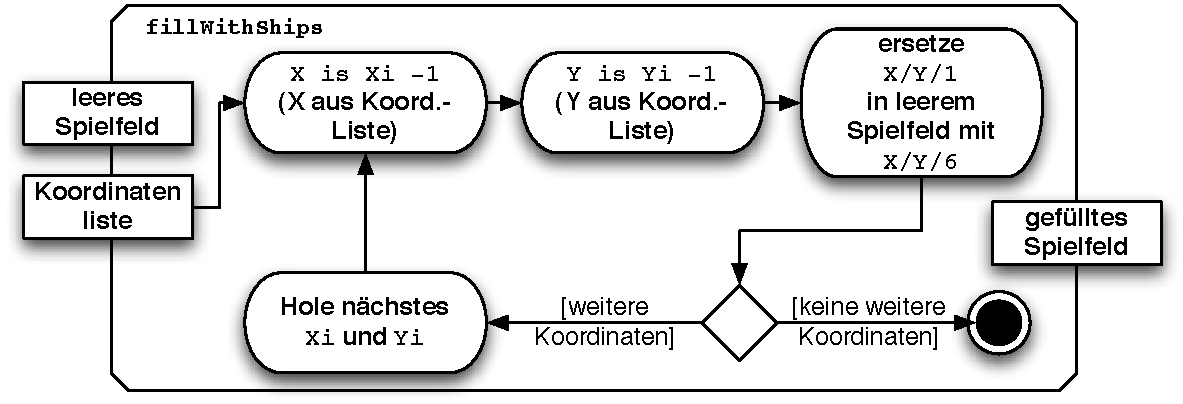
\includegraphics[width=.9\textwidth]{images/fillWithShips.pdf}
		\caption{UML Aktivitätsdiagramm des Prädikats \texttt{fillWithships/3}. \emph{Quelle: Eigene Darstellung.}}
		\label{fig:fillwithShips3}
	\end{figure}
	% figure fig:fillwithShips3 (end)

\subsubsection{Modul zur Plazierung von Schiffen} \label{sec:initships}	
	Die Aufgabe des Positionierungsmoduls \texttt{initShips.pl} ist es, die Schiffe der künstlichen Intelligenz auf dem Spielfeld zu platzieren.
	Hierfür werden in diesem Modul die Regeln zur legalen Positionierung der Schiffe (siehe Abschnitt \ref{sec:Spielregeln}) implementiert. Neben den Regeln 
	zur Platzierung definiert \texttt{initShips.pl} auch die Anzahl und Länge der im Spiel genutzten Schiffe. Des weiteren wurden Prädikate implementiert, 
	welche die Regeln auf die Menge der Schiffe anwenden, um so mögliche Positionierungen dieser auf dem Spielfeld zu erzeugen.
	
	Das Prädikat \texttt{place/1} stößt die Erzeugung einer zufälligen Aufstellung aller Schiffe auf dem Spielfeld an und gibt diese als Liste der Form 
	\texttt{Schiffs-ID}/ \texttt{Teilnummer}/ \texttt{X-Koordinate}/ \texttt{Y-Koordinate} an.
	
	Um sicherzustellen das nur legale Positionierungen verwendet werden, wurden die Spielregeln (siehe Abschnitt \ref{sec:Spielregeln}) wie folgt implementiert:
	\begin{itemize}
		\item Schiffe dürfen Horizontal oder Vertikal auf dem Spielfeld platziert werden.\newline
		\lstinputlisting[firstline=29, lastline=46,
		caption=Implementierung der Platzierungsregel in Prolog,
		label=code:PrologRules1]{includes/initShips.pl}
		\item Verschiedene Schiffe dürfen einander nicht berühren, aber diagonal versetzt stehen.
		\lstinputlisting[firstline=47, lastline=68, 
		caption=Implementierung der Platzierungsregel in Prolog,
		label=code:PrologRules2]{includes/initShips.pl}
	\end{itemize}
	Die Anwendung dieser Regeln erfolgt durch die Abfolge rekursiver Prädikate, welche eine Liste von legal positionierten Schiffen aufbauen. Es wird also 
	erst ein Schiff auf dem Spielfeld positioniert, dann ein Zweites dazu gesetzt, darauf folgt das dritte Schiff und so weiter, bis alle fünf Schiffe Positioniert 
	sind. Um eine möglichst zufällige und unvorhersehbare Positionierung der Schiffe zu erreichen, werden, da wo es möglich ist, Sequenzen von Zufallszahlen anstatt 
	fest kodierter Listen genutzt. Folgendes UML-Diagramm (Abb. \ref{fig:itShips}) stellt den diesen Ablauf schematisch und vereinfacht dar.
	\begin{itemize}
		\item Das \texttt{Template} ist eine Liste, welche die Schiffe und Eigenschaften (die Länge) beschreibt. Für ein fünf Teile langes Schiff, finden sich im 
		Template fünf Elemente der Form \texttt{Schiffs-ID: 1-5}/ \texttt{Teilenummer: 1-5}/ \texttt{X-Koordinate: Variabel}/ \texttt{Y-Koordinate: Variabel}.
		\item Zu Beginn der Positionierung wird die Reihenfolge, in der die Schiffe platziert werden, zufällig festgelegt. Hierfür wird eine zufällige Sequenz der 
		Zahlen 1 bis 5 erzeugt und in der Liste \texttt{ships} gespeichert.
	\end{itemize}
	\begin{figure}[H] % (fold)
		\centering
		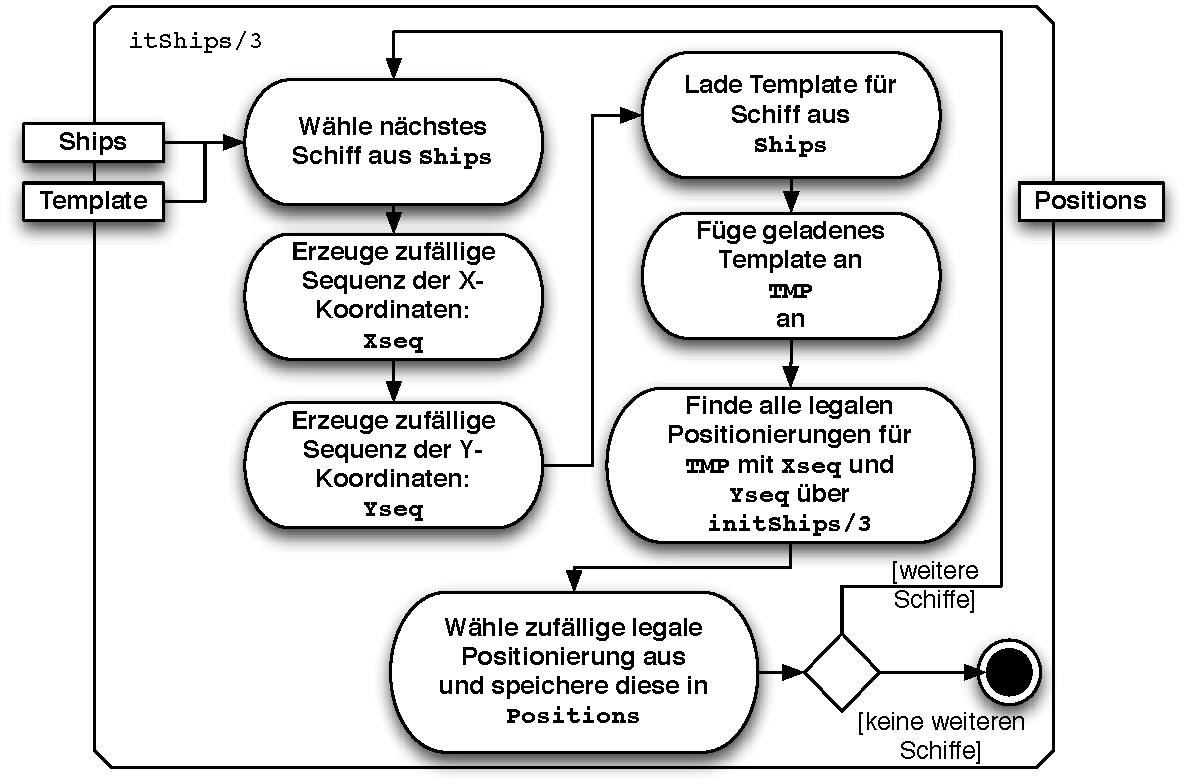
\includegraphics[width=0.9\textwidth]{images/itShips3.pdf}
		\caption{UML-Aktivitätsdiagramm zum Prädikat \texttt{itShips/3}}
		\label{fig:itShips}
	\end{figure}
	% figure fig:initShips (end)
	Auch in \texttt{itShips/3} ist die, in Abbildung \ref{fig:itShips} dargestellte Schleife, als rekursiver Prädikatsaufruf implementiert 
	(vgl. Abschnitt \ref{sec:initModule} und Abbildung \ref{fig:fillwithShips3}).
	
	Das Prädikat \texttt{initShips/3}, welches in Abbildung \ref{fig:itShips} referenziert wird, wendet die in Listing \ref{code:PrologRules1} 
	und \ref{code:PrologRules2} dargestellten 
	Regeln auf die übergebene Liste von Schiffen an. Hierfür werden die übergeben X- und Y-Sequenzen (\texttt{Xseq}, \texttt{Yseq}; die Wertebereiche des Koordinatensystems, 
	welches das Spielfeld abbildet) der Reihe nach abgearbeitet und somit alle legalen Positionierungen für die übergebene Schiffsliste gefunden. Aufgrund der 
	Tatsache, dass immer nur ein Schiff mit Variablen X- und Y-Koordinaten in der übergebenen Liste vorhanden ist (andere, ggf. vorhandene Schiffe, haben bereits 
	in vorherigen durchläufen Koordinaten zugewiesen bekommen), hält sich der Rechenaufwand und die Anzahl der möglichen Positionierungen klein und Prolog kann 
	eine Menge an Lösungen finden und zurückgeben.
\subsubsection{Verteidigungsmodul} \label{sec:defendModule}
	Die Aufgabe des Verteidigungsmoduls \texttt{defendModule.pl} ist es einen Angriff des Gegners zu verarbeiten.
	Zum einen muss dabei der Status des eigenen Feldes \texttt{myField/1} aktualisiert 
	und zum anderen die Antwort für den Gegner bestimmt werden.
	
	Hat der Gegner ins Wasser geschossen, so ist keine Änderung des eigenen Feldes notwendig. Trifft der Gegner jedoch ein Schiff,
	so muss ermittelt werden, ob dieser Treffer das Schiff lediglich getroffen oder sogar versenkt hat. Außerdem ändert sich die Antwort
	für den Gegner, wenn das letzte Schiff versenkt wurde.
	
	Ob das letzte Schiff versenkt wurde, erfolgt mit Hilfe einer Abfrage nach verbleibenden Schiffen (Feldstatus 6) im Prädikat \texttt{myField/1}.
	
	Die Überprüfung, ob ein Schiff vollständig versenkt wurde, erfolgt über eine rekursive Überprüfung der 4 benachbarten Felder.
	Dabei erhöht sich die Rekursionstiefe, wenn ein Nachbarfeld ebenfalls als getroffen markiert ist. 
	Da in den Regeln festgelegt ist, dass Schiffe sich nicht berühren dürfen, kann mit diesem Vorgehen festgestellt werden, ob ein Schiff
	vollständig versenkt wurde, oder sich unter den Nachbarn noch ungetroffene Teile befinden.
	
	Schlägt die zuletzt erläuterte Überprüfung fehl, so wurde nur ein Teil eines Schiffes getroffen. Und die entsprechende Antwort wird zurück 
	gegeben.
	
	
\subsubsection{Angriffsmodul} \label{sec:attackModule}
	Die Aufgabe des Angriffsmoduls \texttt{attackModule.pl} ist es, eine Koordinate für den nächsten Angriff zu liefern und außerdem den 
	Rückgabewert des Angriffs zu verarbeiten. 
	Dafür werden die Prädikate \texttt{doAttack/2} und \texttt{attackResponse/3} verwendet. 
	
	Wird das Prädikat \texttt{doAttack} aufgerufen, so nutzt das Angriffsmodul zunächst das Prädikat \texttt{getPointOfAttack/2} des
	Strategiemoduls, um den als nächstes zu attackierenden Punkt zu erhalten. Anschließend überprüft \texttt{doAttack/2} 
	ob die erhaltene Koordinate im Feld des Gegners \texttt{enemyField/1} als unbekannt (Status 0) gilt (Prädikat \texttt{doAttackCheck}. 
	Ist dies nicht der Fall, so wird eine neue Koordinate von \texttt{getPointOfAttack/2} angefordert. 
	Gilt die Koordinate als unbekannt, so wird dieser Punkt als nächster Angriffspunkt zurück gegeben.
	
	Das Prädikat \texttt{attackResponse/3} verarbeitet die Antwort des Gegners auf einen Angriff. Zum einen wird das intern gehaltene, 
	gegnerische Feld aktualisiert (\texttt{updateEnemyField/3}), zum anderen wird die Openlist für weitere Angriffe über 
	das Prädikat \texttt{updateOpenList/3} aus dem Strategiemodul aktualisiert (siehe Abschnitt \ref{sec:strategy}).
	
	Zur Aktualisierung des gegnerischen Spielfeldes \texttt{enemyField/1} wird der vom Gegener erhaltene Status in das entsprechende 
	Feld eingetragen. Eine Ausnahme besteht für die Antwort \textit{Schiff vollständig versenkt}, in diesem Fall wird das ensprechende
	Feld lediglich mit dem Status \textit{Treffer} belegt, um die Handhabung des Spielfeldes zu erleichtern. 

	\subsubsection{Strategiemodul} \label{sec:strategy}

Das Strategiemodul \texttt{strategy.pl} stellt das Prädikat zur Bestimmung des nächsten Angriffspunktes \texttt{getPointOfAttack/2}	zur Verfügung. 
Außerdem füllt dieses Modul die Liste der priorisiert anzugreifenden Punkte über das Prädikat \texttt{updateOpenList/3}. 

Beim Aufruf von \texttt{getPointOfAttack/2} wird das erste Element der Openlist \texttt{openList/2} zurückgegeben.
Befinden sich keine Koordinaten in der Openlist \texttt{openList/1}, so gibt \texttt{getPointOfAttack/2} einen zufälligen Angriffspunkt zurück.

Das Prädikat \texttt{updateOpenList/3} erhält die angegriffene Koordinate und den vom Gegner erhaltenen Rückgabewert. 
Traf der Angriff Wasser oder das letzte Schiff des Gegners, so wird lediglich die angegriffene Position aus der Openlist gelöscht.

Wurde das gerade attackierte Schiff vollständig versenkt, so kann die aktuelle Openlist vollständig geleert werden, da stets nur ein Schiff attackiert wird. 
Außerdem werden die unmittelbar benachbarten Felder des versenkten Schiffes als \textit{Wasser} markiert, denn aufgrund der Spielregeln darf sich auf diesen Feldern kein weiteres Schiff befinden (Prädikat \texttt{surroundWithWater/4}). 

Ist die Antwort des Gegeners \textit{Treffer}, so muss die Openlist aktualisiert werden. 
Dazu werden zunächst alle benachbarten Felder in die Openlist eingetragen, deren Status unbekannt ist (Prädikat \texttt{appendFreeFieldToList/2}). 

Als mögliche Kandidaten der Openlist gehen die Felder der direkten 4er-Nachbarschaft des Treffers ein, wie es in Abbildung \ref{fig:ErstelleOpenlist} zu sehen ist.
Die Reihenfolge wurde auf Westen, Osten, Norden, Süden festgelegt.
\begin{figure}[H]
  \centering
  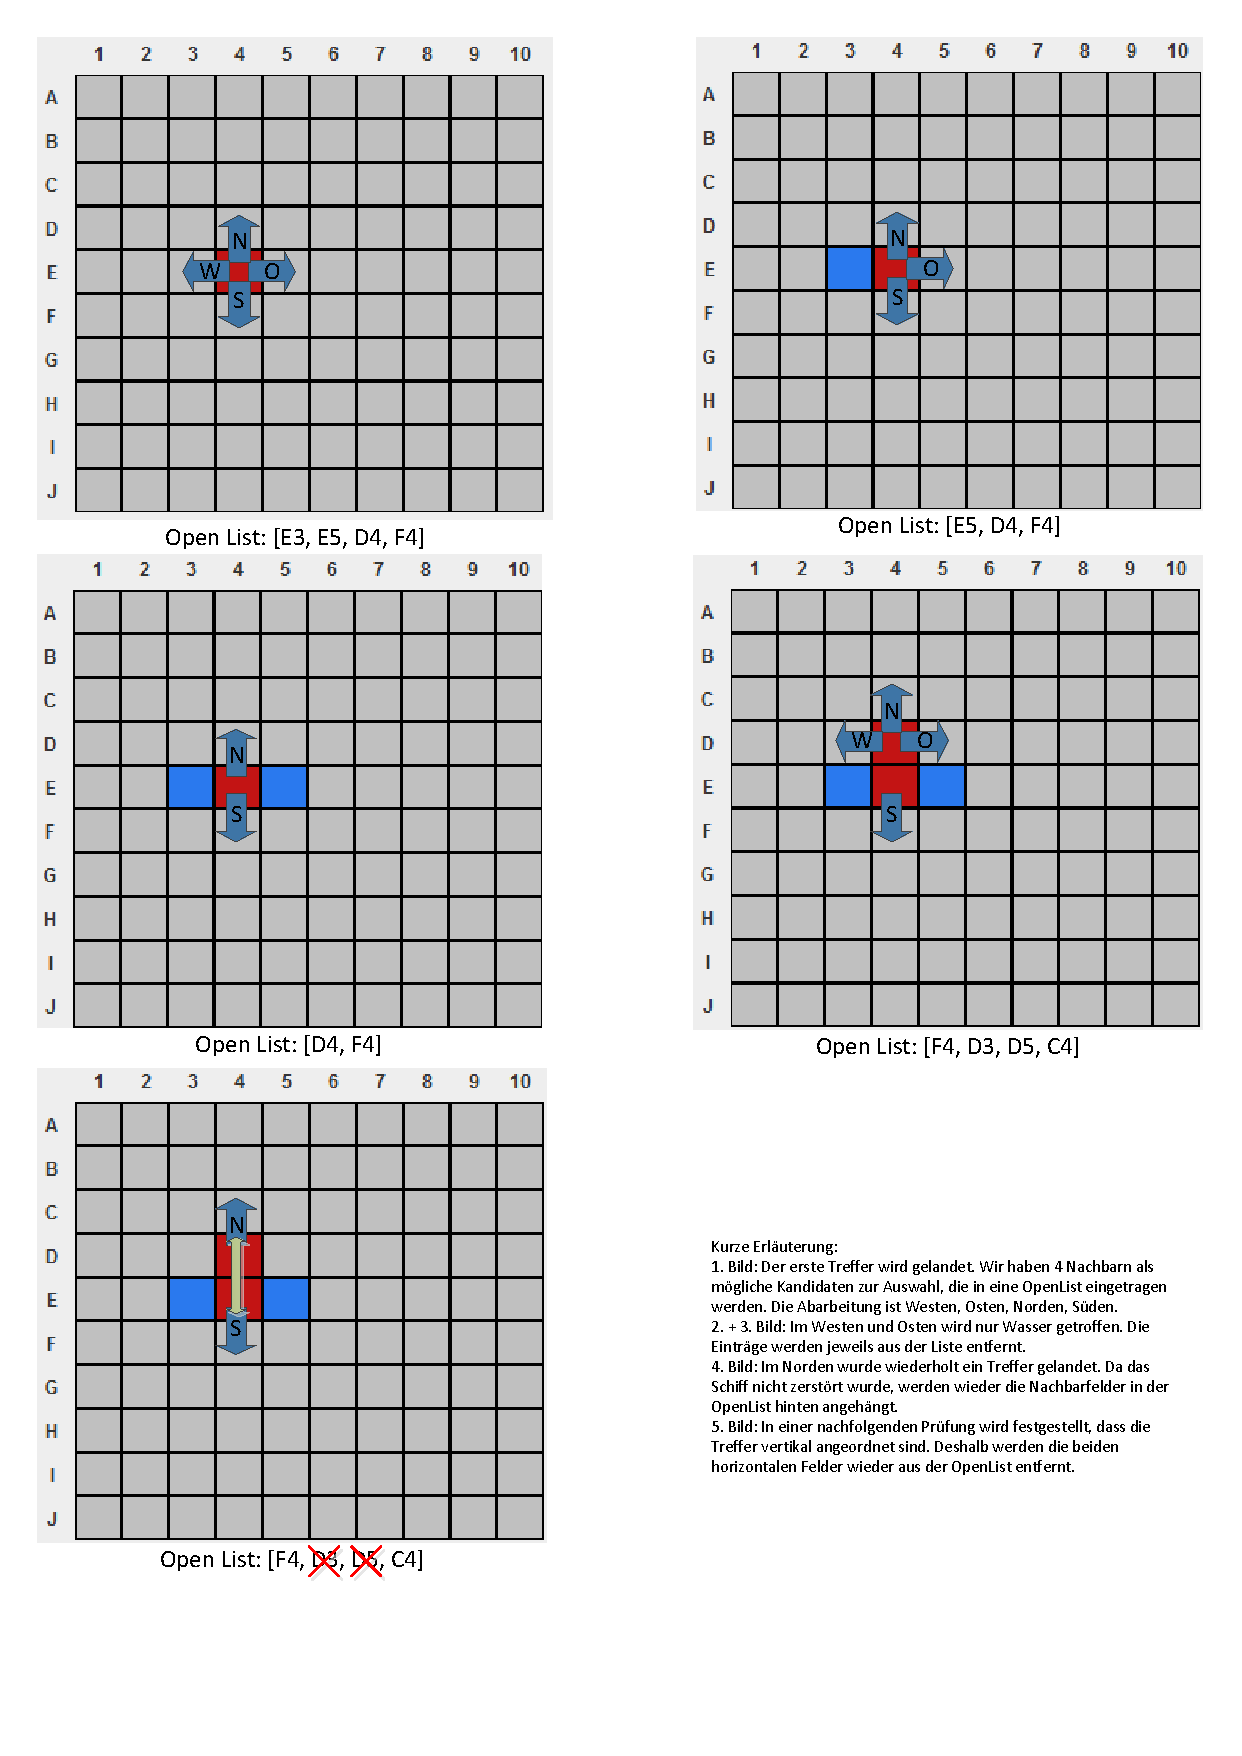
\includegraphics[trim=5mm 204mm 105mm 4mm,clip,width=0.5\textwidth]{images/Strategie_1_FirstHit.pdf}
  \caption{Openlist mit benachbarten Feldern initialisieren}
  \label{fig:ErstelleOpenlist}
\end{figure}

In den nachfolgenden Spielzügen werden diese Felder geprüft.
Sollten diese sich als "'Wasser"' herausstellen, wie es in der Abbildung \ref{fig:Openlist2} angedeutet ist, so werden die entsprechenden Einträge ohne weitere Verarbeitung aus der Openlist gelöscht.
\begin{figure}[H]
  \centering
  \subfigure[Westen (verfehlt)]{
    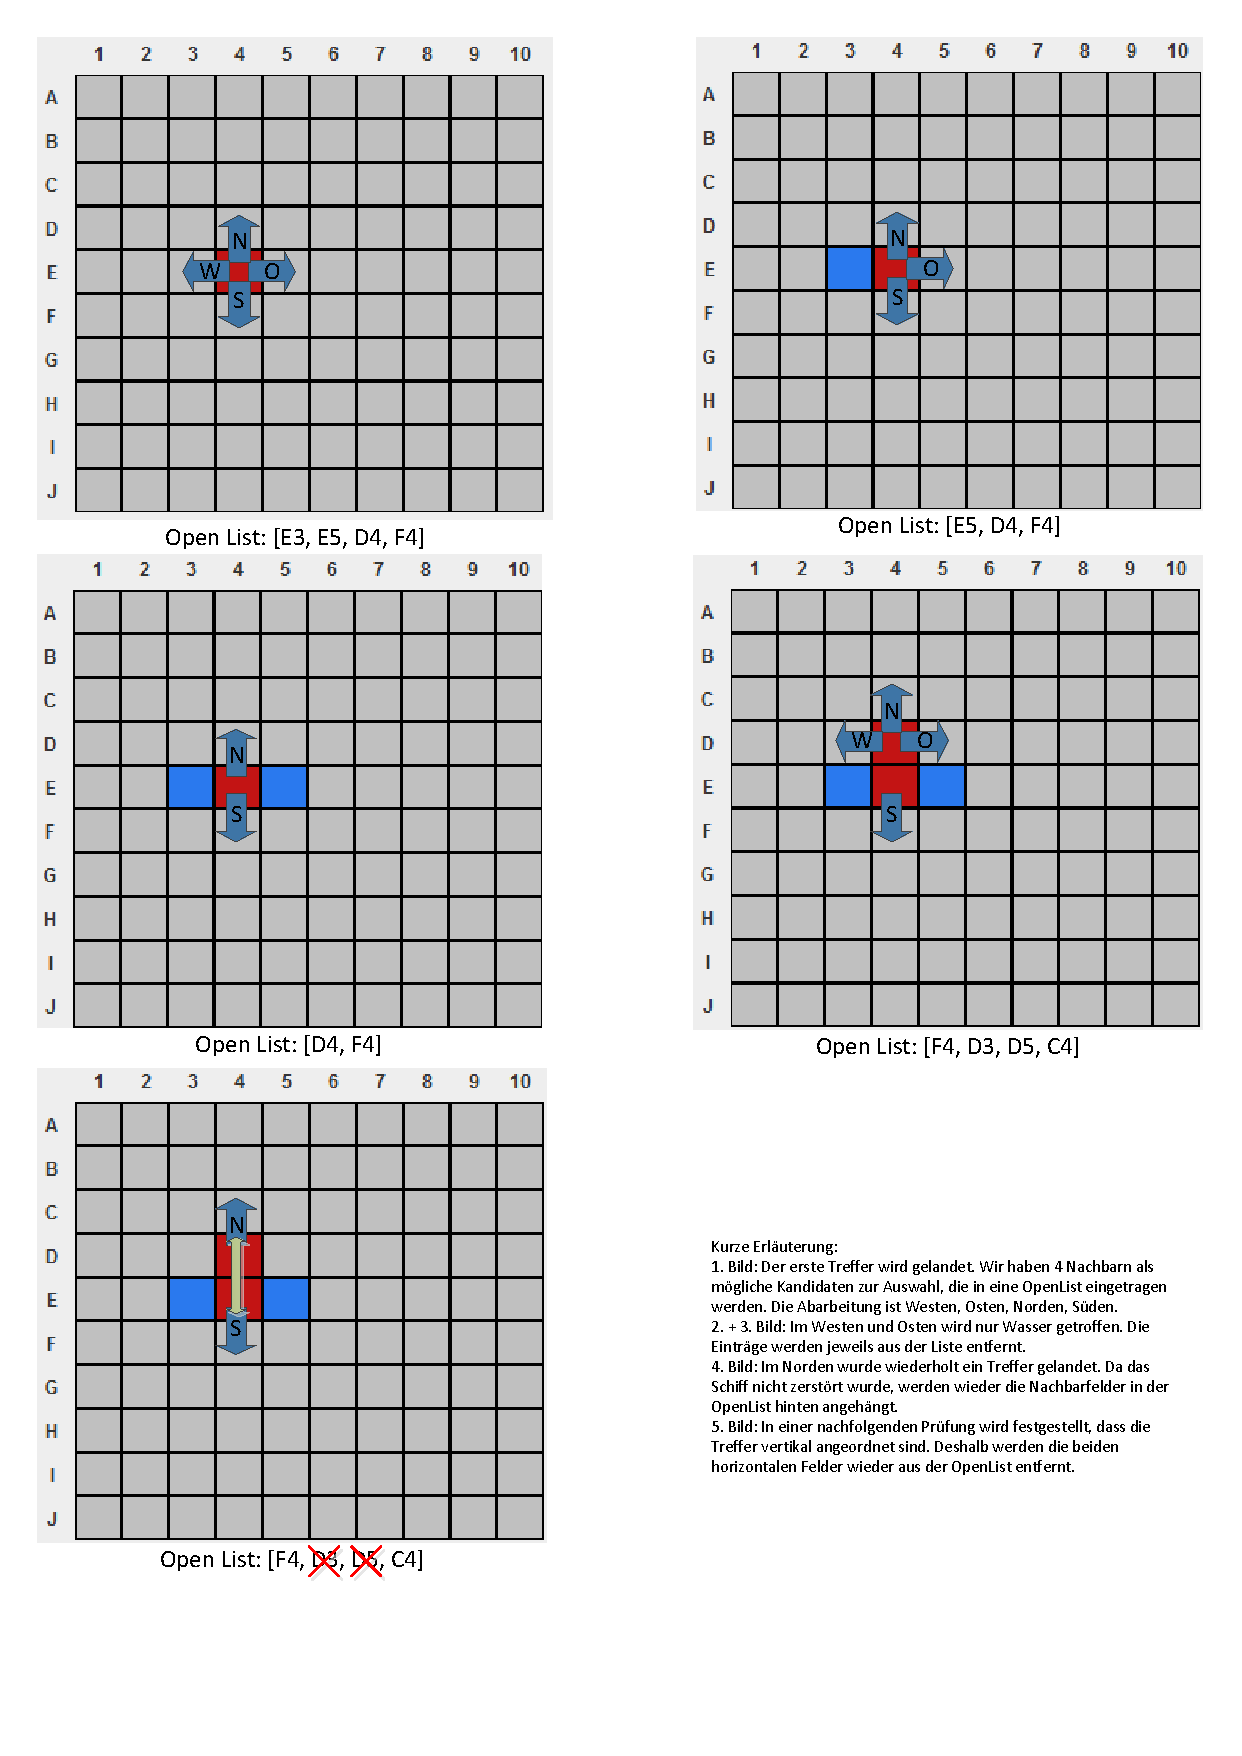
\includegraphics[trim=105mm 204mm 5mm 4mm,clip,width=0.47\textwidth]{images/Strategie_1_FirstHit.pdf}
    \label{fig:west}
  }
  \subfigure[Osten (verfehlt)]{
	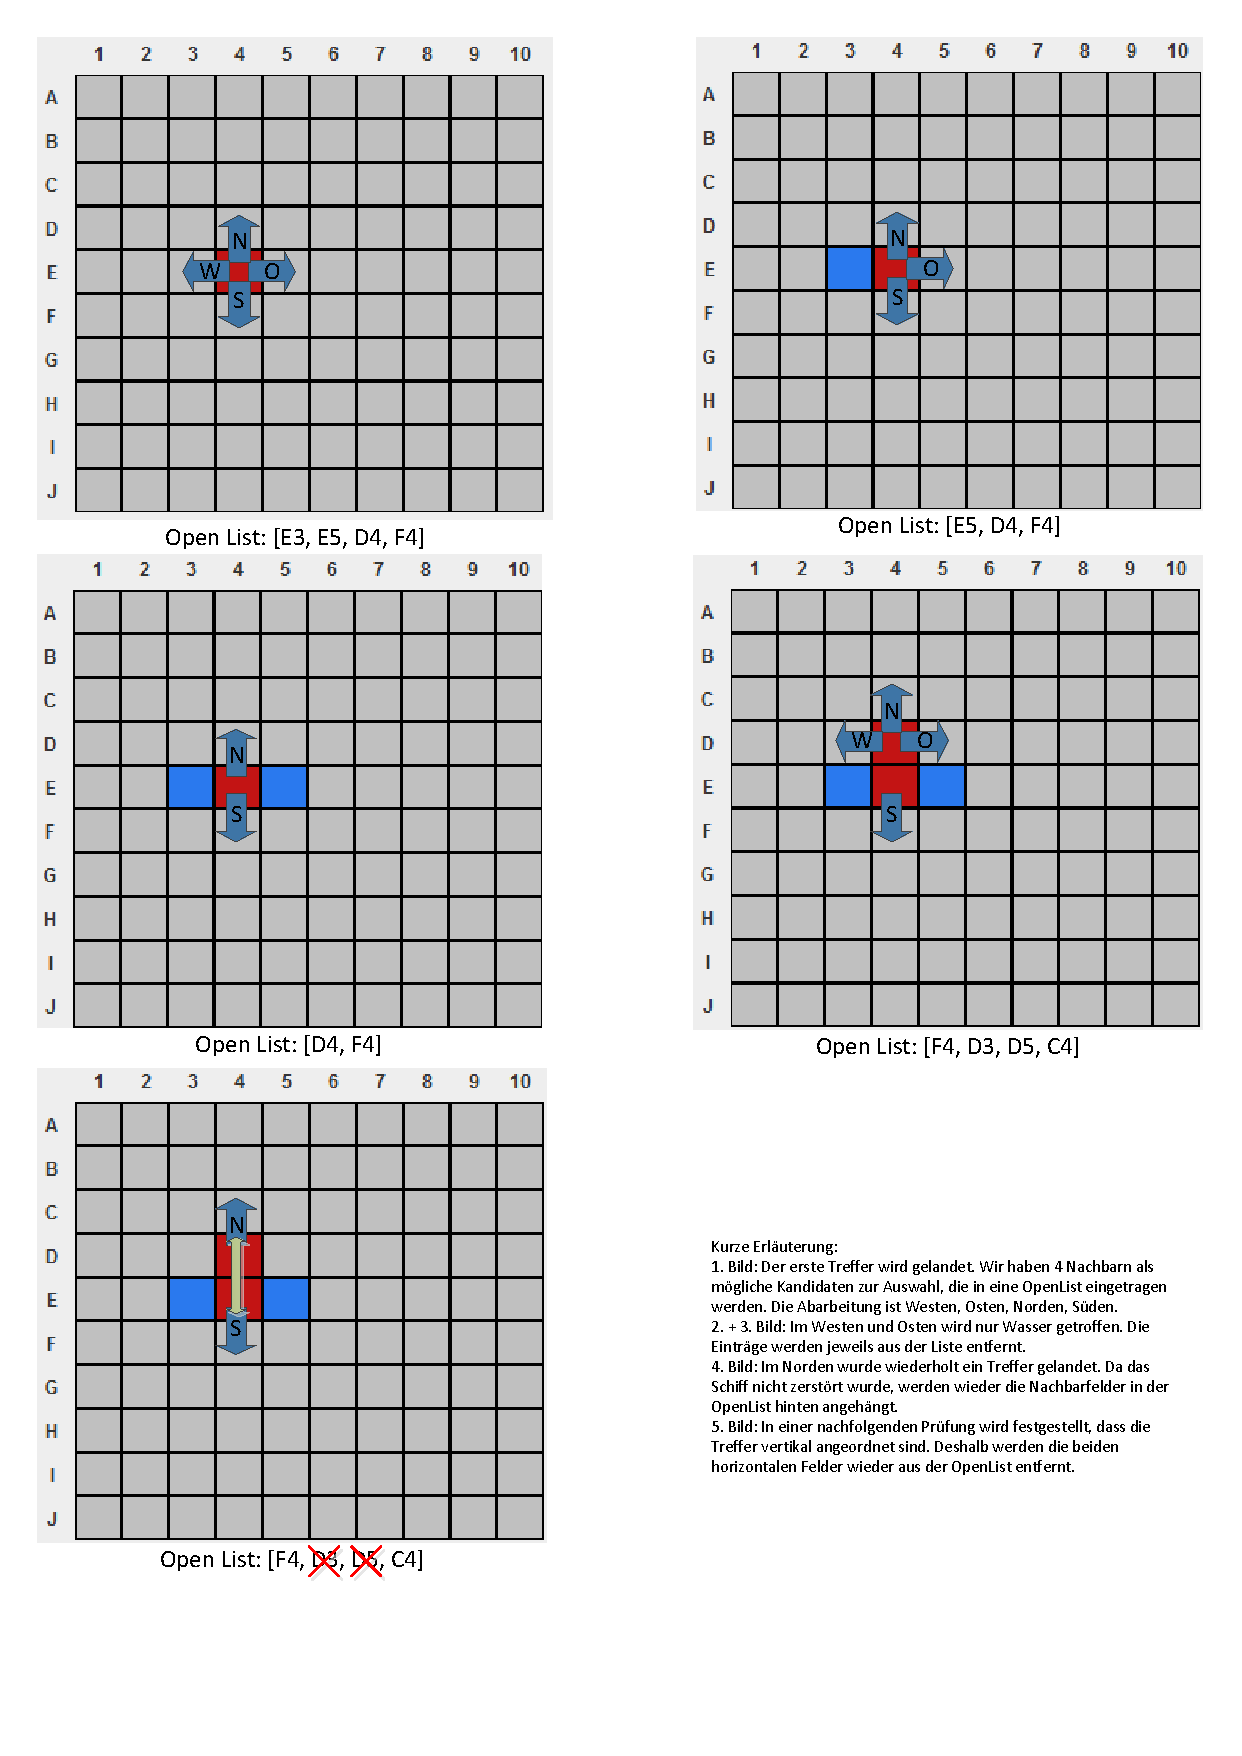
\includegraphics[trim=5mm 117mm 105mm 94mm,clip,width=0.47\textwidth]{images/Strategie_1_FirstHit.pdf}
    \label{fig:east}
  }
  \caption{Openlist nach zwei misglückten Angriffen}
  \label{fig:Openlist2}
\end{figure}

Im Falle eines weiteren Treffers wiederholt sich der Algorithmus und nimmt alle unbekannten und benachbarten Felder des Treffers in die Openlist auf (vgl. Abbilidung \ref{fig:north}).
Anschließend wird mit dem Prädikat \texttt{checkHitDirection/2} überprüft, ob die Orientierung des attackierten Schiffes (horizontal oder vertikal) bereits durch frühere Treffer bekannt ist. 
Ist dies der Fall, so kann die Openlist entsprechend um auszuschließende Positionen verkürzt werden.
Im hier gezeigten Beispiel können die horizontalen Felder $D3$ und $D5$ wieder aus der Liste gestrichen werden.
\begin{figure}[H]
  \centering
  \subfigure[Norden (Treffer)]{
    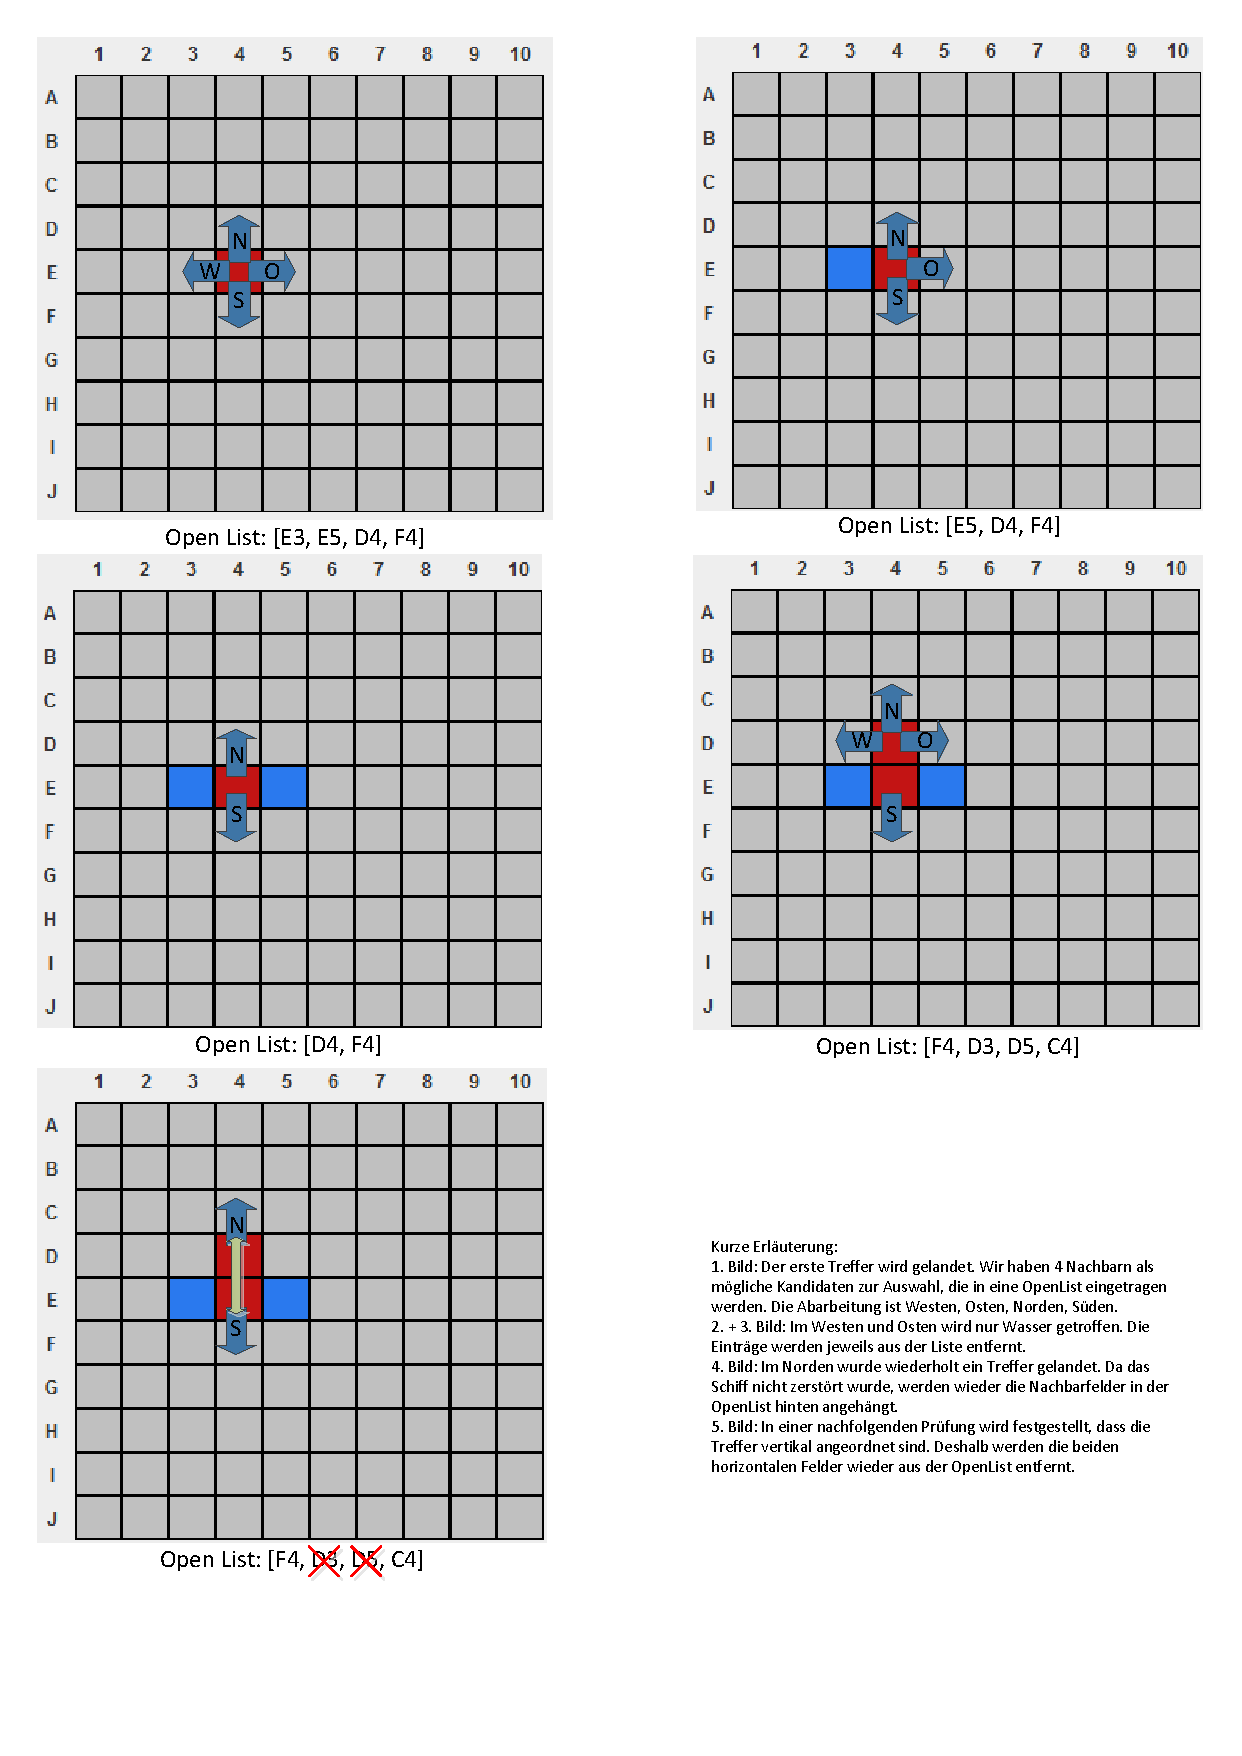
\includegraphics[trim=105mm 117mm 5mm 94mm,clip,width=0.47\textwidth]{images/Strategie_1_FirstHit.pdf}
    \label{fig:north}
  }
  \subfigure[Bereinigte Openlist]{
	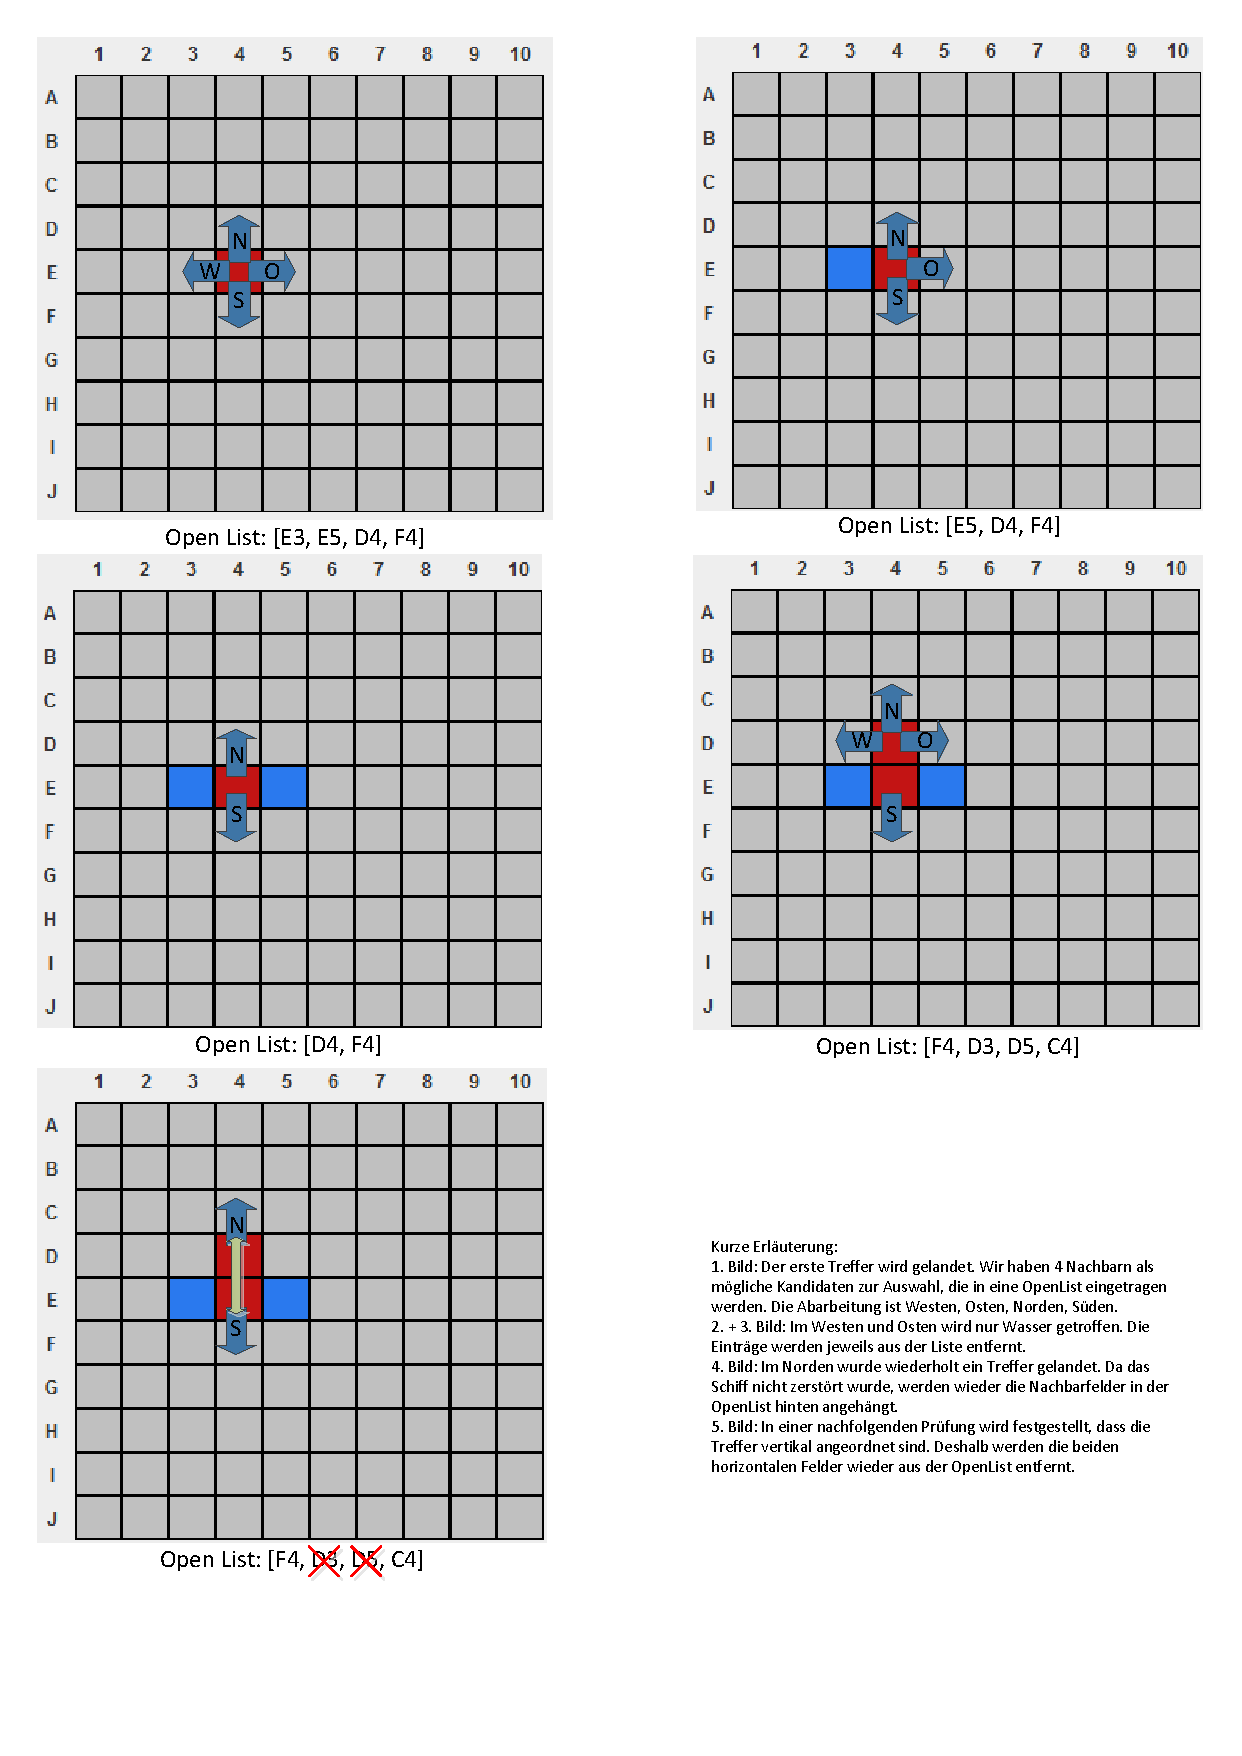
\includegraphics[trim=5mm 30mm 105mm 180mm,clip,width=0.47\textwidth]{images/Strategie_1_FirstHit.pdf}
    \label{fig:northupd}
  }
  \caption{Aktualisierung der Openlist nach einem Treffer}
  \label{fig:Openlist3}
\end{figure}

Nachdem das Schiff vollständig zerstört wurde, wird die Openlist geleert und die Auswahl der anzugreifenden Koordinaten erfolgt wieder solange zufällig, bis der nächste Treffer erzielt wurde.
% \subsubsection{Strategiemodul} \label{sec:strategy}

	% Das Strategiemodul \texttt{strategy.pl} stellt das Prädikat zur Bestimmung des nächsten Angriffspunktes \texttt{getPointOfAttack/2}
	% zur Verfügung. Außerdem füllt dieses Modul die Liste der priorisiert anzugreifenden Punkte über das Prädikat \texttt{updateOpenList/3}. 
	
	% Beim Aufruf von \texttt{getPointOfAttack/2} wird das erste Element der Openlist \texttt{openList/2} zurückgegeben.
	% Befinden sich keine Koordinaten in der Openlist \texttt{openList/1}, so gibt \texttt{getPointOfAttack/2} einen zufälligen Angriffspunkt zurück.
	
	% Das Prädikat \texttt{updateOpenList/3} erhält die angegriffene Koordinate und den vom Gegner erhaltenen Rückgabewert. 
	% Traf der Angriff Wasser oder das letzte Schiff des Gegners, so erfolgt keine Änderung der Openlist.
	
	% Wurde das gerade attackierte Schiff vollständig versenkt, so kann die aktuelle Openlist vollständig geleert werden, da stets nur ein 
	% Schiff attackiert wird. Außerdem werden die unmittelbar benachbarten Felder des versenkten Schiffes als \textit{Wasser} markiert, denn
	% Aufgrund der Spielregeln darf sich auf diesen Feldern kein weiteres Schiff befinden (Prädikat \texttt{surroundWithWater/4}). 
	
	% Ist die Antwort des Gegeners \textit{Treffer}, so muss die OpenList aktualisiert werden. 
	% Dazu werden zunächst alle benachbarten Felder in die Openlist eingetragen, deren Status unbekannt ist 
	% (Prädikat \texttt{appendFreeFieldToList/2}). 
	% Anschließend wird mit dem Prädikat \texttt{checkHitDirection/2} überprüft, ob die Orientierung 
	% des attackierten Schiffes (horizontal oder vertikal) bereits durch frühere Treffer bekannt ist. 
	% Ist dies der Fall, so kann die Openlist entsprechend um auszuschließende Positionen verkürzt werden.

\subsubsection{Ausgabemodul}
		Das Ausgabemodul \texttt{outputModule.pl} beinhaltet Prädikate zur Ausgabe der \textit{globalen Variablen} \texttt{myField/1},
		\texttt{enemyField/1} sowie \texttt{openList/1}. Die Ausgabe erfolgt standardgemäß auf der Standardausgabe und kann während des Spiels oder zu
		Debugzwecken verwendet werden.

		Um Eine Überflutung der Ausgabekonsole bei vielen automatisierten Spieldurchläufen (zum Beispiel: KI gegen KI, 1000 spiele) zu vermeiden, kann 
		die Ausgabe über das Prädikat \texttt{verbose/1} gesteuert werden (siehe Abschnitt \ref{ssub:ausgabeverhalten}).
\subsubsection{Ausgabeverhalten} % (fold)
\label{ssub:ausgabeverhalten}
		Das Modul \texttt{verbosity.pl} steuert den Ausgabekanal, auf dem während des Spielens Debug-Informationen dargestellt werden können. 
		Es sind drei verschiedene Ausgabeverhalten implementiert:
			\begin{enumerate}
				\item \texttt{verbose(0)} : Keinerlei Ausgabe während des Spiels.
				\item \texttt{verbose(1)} : Ausgaben während des Spiels werden in eine Textdatei umgeleitet.
				\item \texttt{verbose(2)} : Ausgaben während des Spiels erscheinen auf der Konsole.
			\end{enumerate}
			Bei allen Modi wird nach Beendigung aller konfigurierten Spiele, eine Zusammenfassung der Ergebnisse auf der Ausgabekonsole ausgegeben.

			Zur Realisierung der verschiedenen Ausgabemodi wird der Standardausgabestrom der SWI-Prolog Umgebung über das Systemprädikat \texttt{set\_output/1} 
			geändert. Die Implementierung von \texttt{verbose/1} findet sich in \texttt{verbosity.pl}. Hier wird je nach Argument ein anderer Ausgabestrom 
			definiert und als Standardausgabestrom gesetzt:
			\begin{itemize}
				\item \texttt{verbose(0)} : erzeugen eines Null-Stroms per \texttt{open\_null\_stream/1}.
				\item \texttt{verbose(1)} : erzeugen eines Ausgabestroms in die Datei "'Output.txt"' im Unterordner "'GameLogs"' per \texttt{open/3}.
				\item \texttt{verbose(2)} : erzeugen eines Ausgabestroms auf die Ausgabekonsole per \texttt{user\_output/0}.
			\end{itemize}
			Nach dem Erzeugen des jeweiligen Ausgabestroms wird dieser über das Systemprädikat \texttt{set\_output} gesetzt und der aktuelle Ausgabestrom 
			im globalen Prädikat \texttt{currentStream/1} gesetzt, sodass er überall im Programm manipuliert werden kann.
			Vor Ausgabe der Spielzusammenfassung wird der momentane Ausgabestrom über das oben beschriebene Prädikat \texttt{currentStream/1} geholt und 
			über das Systemprädikat \texttt{close/1} geschlossen. Direkt danach wird \texttt{verbose(2)} gesetzt, sodass die Ausgabe 
			der Zusammenfassung in jedem Fall auf der Ausgabekonsole erscheint.
% subsubsection ausgabeverhalten (end)
	

